
\newpage 

\section{New potential and repulsive Coulomb interaction}

Until now the considered potential has been described by $\rho^2$ for one particle. When introducing another particle the potential is changed so the new potential is given by \matref{eq:Newpotential}, where $\omega$ is an oscillator frequency and $\frac{1}{\rho}$ is a repulsive Coulomb potential.
\begin{equation}
V_{\rho} = \omega^2\rho^2 + \frac{1}{\rho}
\label{eq:Newpotential}
\end{equation}

First considering the case without a repulsive Coulumb interaction. The aim is finding a value of $\rho_{max}$ so that the eigenvalues are considered stable.  
%----------------------------------
\begin{wraptable}{r}{5.0cm}
\caption{Table for finding best $\rho_{max}$ looking at the 1st eigenvalue} 
\label{tab:rhomax}
\phantom{.}
\begin{tabular}{|c|c|c|}
\hline
$\rho_{max}$ & N & 1st eigenvalue \\
\hline 
1 & 10 & 9.80273 \\
2 & 20 & 2.46292 \\
3 & 30 & 1.09594 \\
4 & 40 & 0.617001 \\
\vdots & \vdots & \vdots \\
9 & 90 & 0.124119\\
10 & 100 & 0.101504 \\
10.1 & 101 & 0.0996154 \\
11 & 110 & 0.0849622 \\
\hline

\end{tabular}

\end{wraptable}
%------------------------------------
For this to be stable the change should be small, so $\rho_{max} = 10$ and the change is about 0.02 between the surrounding steps. Also the change between 10 and 10.1 is about 0.002 so small changes in $\rho_{max} $ doesn't give big changes. Also the relation between $\rho_{max}$ and n is kept constant so that h is constant. Running for different values of $\rho_{max}$ with the ratio gives \tabref{tab:rhomax}, which shows that when $\rho_{max} $ is 10 the results are stable for the 1st eigenvalue. 


The Eigenvectors are used for determining the wave function, and in this case they are used squared so they show the probability density of the distance $\rho$ between the two electrons. Which gives the most probable distance between the particles,the distance $\rho = (\frac{1}{\alpha})r$ where $\alpha = (\frac{\hbar^2}{mk})^{1/4}$ is the Bohr radius. This is described in \secref{sec:NatureOfTheProblem}. And only the ground state is considered. Plotting the distance as a function of $\rho$ for different values of the frequency $\omega_r$, \figref{fig:ProbFuncOmegaWithout} shows that for a higher frequency $\omega_r$ the distance between the particles are bigger and the spread in area which the particle can be in is also more stretched out. 

\begin{figure}[H]
	\centering
	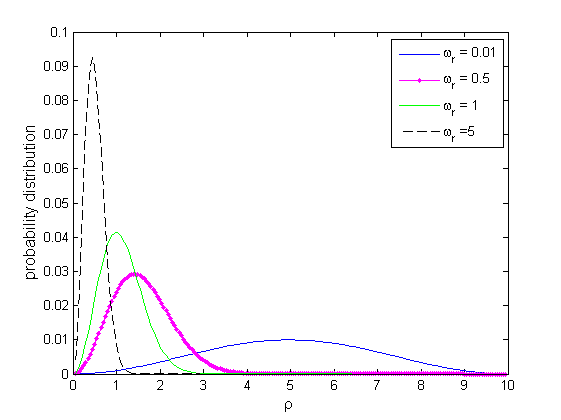
\includegraphics[width=0.75\textwidth]{Figures/2particles_without.png}
	\caption{The probability density as a function of distance $\rho$ without repulsive Coulomb interaction. Where $\rho_{min} = 0$, $\rho_{max} = 10$ and $n = 200$  }
	\label{fig:ProbFuncOmegaWithout}
\end{figure}

When adding a repulsive Coulomb potential $\frac{1}{\rho}$ to the potential $V(\rho )$ in \figref{fig:ProbFuncOmega} the probability density is pushed to a longer distance, although it might be a bit difficult to see in \figref{fig:ProbFuncOmega} and \figref{fig:ProbFuncOmegaWithout}. Physically it makes sense that the repulsive Coulomb interaction should increase the distance between the electrons as it gives a greater contribution when the electrons are close. The choice of $\rho$ is good because most of the probability distribution is inside the distance $\rho$. Also if there is no repulsive Coulomb interaction and the frequency $\omega = 1$ then the system acts as in the one particle case, and the choice of $\rho_{max} = 5$ there includes  most of the particle distributions. 

\begin{figure}[H]
	\centering
	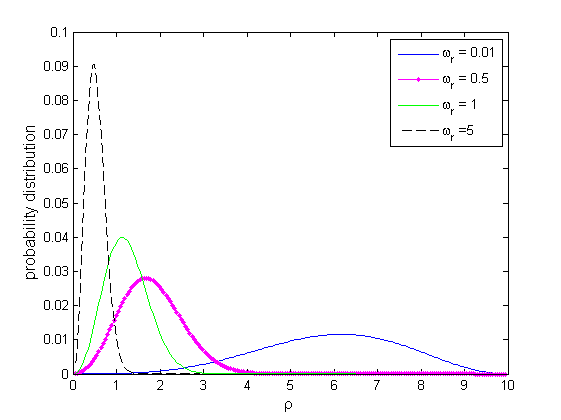
\includegraphics[width=0.75\textwidth]{Figures/ProbFuncOmega.png}
	\caption{The probability density as a function of distance $\rho$ with a repulsive Coulomb interaction. Where $\rho_{min} = 0$, $\rho_{max} = 10$ and $n = 200$}
	\label{fig:ProbFuncOmega}
\end{figure}





